\documentclass[
%a4paper,12pt
encoding=utf8
]{../twoeskd}

% \usepackage{eskdappsheet}

% Packages required by doxygen
\usepackage[export]{adjustbox} % also loads graphicx
\usepackage{graphicx}
\usepackage[utf8]{inputenc}
\usepackage{multicol}
\usepackage{multirow}
\usepackage{makeidx}

% NLS support packages
\usepackage[T2A]{fontenc}
\usepackage[russian]{babel}
\usepackage{pscyr}

% Font selection
\usepackage{courier}
\usepackage{amssymb}

\setlength{\parindent}{0cm}
\setlength{\parskip}{0.2cm}

% debug to see the frame borders
% from https://en.wikibooks.org/wiki/LaTeX/Page_Layout
% \usepackage{showframe}

% Indices & bibliography
\usepackage{natbib}
\usepackage[titles]{tocloft}
\setcounter{tocdepth}{3}
\setcounter{secnumdepth}{5}

% change style of titles in \section{}
\usepackage{titlesec}
\titleformat{\section}[hang]{\huge\bfseries\center}{\thetitle.}{1em}{}
\titleformat{\subsection}[hang]{\Large\normalfont\raggedright}{\thetitle.}{1em}{\underline}
\titleformat{\subsubsection}[hang]{\large\normalfont\raggedright}{\thetitle.}{1pt}{}

% Packages for text layout in normal mode
% \usepackage[parfill]{parskip} % автоматом делает пустые линии между параграфами, там где они есть в тексте
% \usepackage{indentfirst} % indent even in first paragraph
\usepackage{setspace}	 % controls space between lines
\setstretch{1} % space between lines
\setlength\parindent{0.9cm} % size of indent for every paragraph
\usepackage{csquotes}% превратить " " в красивые двойные кавычки
\MakeOuterQuote{"}


% this makes items spacing single-spaced in enumerations.
\newenvironment{my_enumerate}{
\begin{enumerate}
  \setlength{\itemsep}{1pt}
  \setlength{\parskip}{0pt}
  \setlength{\parsep}{0pt}}{\end{enumerate}
}


% Custom commands
% configure eskd
\titleTop{
\textbf{\Large ПРАВИТЕЛЬСТВО РОССИЙСКОЙ ФЕДЕРАЦИИ \\
НАЦИОНАЛЬНЫЙ ИССЛЕДОВАТЕЛЬСКИЙ УНИВЕРСИТЕТ \\
«ВЫСШАЯ ШКОЛА ЭКОНОМИКИ» } \\
\vspace*{0.2cm}
{\small Факультет компьютерных наук \\
Департамент программнoй инженерии \\
}
}
\titleDesignedBy{Студент группы БПИ 151 НИУ ВШЭ}{Абрамов А.M.}
\titleAgreedBy{%
\parbox[t]{7cm} {
Доцент департамента \\
программной инженерии \\
факультета компьютерных наук \\
канд. техн. наук \\
}}{Ахметсафина Р. З.}
\titleApprovedBy{
\parbox[t]{10cm} {
Академический руководитель \\
образовательной программы \\
«Программная инженерия» \\
профессор департамента программной \\
инженерии канд. техн. наук \\
}}{Шилов В. В.}
\titleName{ПРОГРАММА СКЕЛЕТНАЯ АНИМАЦИЯ}
\workTypeId{RU.17701729.509000 T3 01-1}

\titleSubname{Техническое задание}


%===== C O N T E N T S =====


\begin{document}

% Titlepage & ToC
\pagenumbering{roman}

% some water filling text, that is pointless but adds text
% \input{annotation}

\newpage
\pagenumbering{arabic}
\tableofcontents

% --- add my custom headers ---
\newpage
\section{Введение}
\subsection{Наименование}
Наименование: «Программатор микроконтроллеров PIC на основе Orange PI Lite». \\
Наименование на английском: «Programmer for PIC Microcontrollers Based on Orange PI Lite». \\


\subsection{Краткая характеристика}
    Цель работы - реализовать программатор для микроконтроллеров PIC серии 16F на тонком клиенте Orange PI Lite.
    В задачи работы входит расчет и инженерия электронной схемы для программирования, написание программы для управления этой схемой.
    Электронная схема предоставляет возможность подключить микроконтроллер PIC серии 16F к тонкому клиенту Orange Pi Lite, управлять уровнями вольтажа на 5В и на 3В и возможность проверить процесс программирования на светодиодах.         
    Программа предоставляет пользователю командный и графичексий интерфейсы, чтение файлов INTEL HЕХ8М, возможность записать файлы программы в программную и EEPROM память микроконтроллера.
    В состав работы также входит создание демонстрационных исходных данных (файлов) для данного программатора и микроконтроллеров серии 16F.

\smallskip
Файл программы в формате INTEL HEX8M, удовлетворяющий требованиям входных данных, может быть получен в результате компиляции исходного кода одним из компиляторов для микроконтроллеров серии PIC 16F. Обычно для разработки используются пакеты предоставляющие интегрированную среду разработки. Например пакет MPLAB X (https://www.microchip.com/, разработчик: организация Microchip Ltd.)


\newpage
\section{Основания для разработки}
\subsection{Документ, на основании которого ведется разработка}
Разработка программы ведется на основании приказа 
\textnumero 6.18.1-02/1112-19 от 11.12.2015 
«Об  утверждении  тем,  руководителей  курсовых  работ  студентов
образовательной  программы  Программная  инженерия 
факультета 
компьютерных наук» в соответствии с учебным планом подготовки бакалавров по направлению «Программная инженерия», факультета Компьютерных наук,
Национального исследовательского университета «Высшая школа экономики» 


\subsection{Наименование темы разработки}
Наименование: «Программатор микроконтроллеров PIC на основе Orange PI Lite». \\
Наименование на английском: «Programmer for PIC Microcontrollers Based on Orange PI Lite». \\


\newpage
\section{Назначение разработки}
\subsection{Функциональное назначение}
Функциональным назначением программы и электронной схемы является предоставление пользователю возможности загрузить программу из файла INTEL HEX8M (.hex), проинтерпретировать полученную информацию, проверить ее на наличие ошибок, стереть программную память и EEPROM память имикроконтроллера, записать прочитанные данные из файла в программную память микроконтроллера, записать новые данных в EEPROM память микроконтроллера без стирания программной памяти. 

\subsection{Эскплутационное назначение}
Программа и электронная схема предназначена для работы на тонком кленте Orange Pi Lite с операционной системой семейства Linux. Программа и схема могут использоваться в учебных целях для демонстации основных компонентов необходимых для прошивки микроконтроллера. Они предоставляют новое направление использования тонкого клиента Orange Pi Lite. Ими может воспользоваться любой человек, желающий запрограммировать микроконтроллер, не имеющий на руках официального программатора, но у которого есть Orange Pi Lite. Данная программа и электронаня схема могут использоваться в качестве дешевой, простой и быстрой алтернативы к покупке официального программатора.


\newpage
\section{Требования к программному изделию}


%=========================================
\subsection{Требования к функциональным характеристикам}
\subsubsection{Требования к составу выполняемых функций}
\begin{my_enumerate}
\item Чтение данных из формата INTEL HEX8M для хранения программы прошивки.
\item Возможность отдельной записи EEPROM памяти, не стирая програмную память микроконтроллера.
\item Поддержка 3 линеек микроконтроллеров серии 16F: 627A / 628A / 648A.
\item Проверка входного файла на корректность.
\item Графический интерфейс для оперирования программой.
\item Интерфейс командной строки для оперирования программой.
\item Повышаюший переходник с 3.3В на 5В для взаимодействия с микроконтроллером.
\item Схемотехника для платы которая позволяет подключить микроконтроллер к тонкому клиенту Orange Pi Lite.
\item Завершенные, работающие схемы на макетной плате.
\item Схемы разводки макетной платы для подключения микроконтроллера к Orange Pi Lite. 
\end{my_enumerate}

\subsubsection{Требования к организации входных и выходных данных}
Входными данными для работы программатора являются скомпилированный файл программы, микроконтроллер подключенный к плате, а также (для обеспечения взаимодействия с пользователем) клавиатура и/или мышь. Входной файл данных может быть созданн в любой среде разработки и любым компилятором поддершивающим формат INTEL HEX8M. Примером такой среды разработки является MPLAB X (https://www.microchip.com/, разработчик: коммерческая организация Microchip Ltd.).

\begin{my_enumerate}
\item Из-за огромного количества серий микроконтроллеров поддерживать их все не представляется возможным. Поэтому программа должна работать только с микроконтроллерами PIC серии 16F, конкретно с линейками 627A / 628A / 648A.
\item Файл программы должен соответствовать формату INTEL HEX8M. По сравнению с двумя другими часто встречающимися форматами INTEL HEX8S, INTEL HEХ32, данный формат наиболее оптимально подходит под серию 16F. В силу того что память 14-битных микроконтроллеров не превышает 64 килобайт (здесь подходит формат HEX32) и програмное слово не нуждаеться в разбиении на высокий и низкий байт как в 16-битных микроконтроллерах (здесь подходит формат HEX8S).
\item Пользователь должен иметь возможность модифицировать следующие входные данные в процессе работы программы в усливиях графического интерфейса и перед запуском программы в командной строке:
\begin{my_enumerate}
\item Указать что требуется запись EEPROM памети без модификации програмной памяти микроконтроллера.
\item Указать что требуется проверить входной файл на ошибки.
\item Указать что требуется записать входной файл в програмную память и в EEPROM память микроконтроллера.
\item Поменять уровень колличества сообщений выводимих программой пользователю.
\item Отменить процесс программирования.
\end{my_enumerate}
\end{my_enumerate}

\medskip
Выходными данными для программатора является запрограммированный микроконтроллер, данные на экране и индикатор программирования на плате программатора.


\subsubsection{Прочие требования}
\begin{enumerate}
\item Поддержка изменения размеров окна.
\item Использование Qt для создания интерфейса.
\end{enumerate}

%=========================================
\subsection{Требования к временным характеристикам}
\begin{enumerate}
\item Задержка между сигналом к началом программирования не должна быть меньше чем 0.001 секунда и не должна превышать 0.1 секунд для файлов программ размером меньше чем 5 килобайт.
\end{enumerate}


%=========================================
\subsection{Требования к интерфейсу}
Интерфейс должен быть прост в использовании. Он должен предоставлять возможность
\begin{my_enumerate}
\item Прочитать данные из формата INTEL HEX8M для хранения программы прошивки.
\item Возможность запрограммировать EEPROM память, не стирая програмную память микроконтроллера.
\item Проверить входной файл на корректность.
\end{my_enumerate}

Командный интерфейс должен предоставлять те же возможности что и графический интерфейс и следовать стандартам принятым при создании интерфейсом командной строки в системе Linux.

%=========================================
\subsection{Требования к надежности}
\subsubsection{Обеспечение устойчивого функционирования программы}
Программа не должна вне зависимости от входных данных или действий оператора завершатся аварийно. При некорректно введенных параметрах пользователю должно отображаться сообщение об ошибке.
\subsubsection{Время восстановления после отказа}
Требования к восстановлению после отказа не предъявляются.
\subsubsection{Отказы из-за некорректных действий оператора}
В случае открытия файла, не соответствующему требованиям ко входным данным, пользователю должно отображаться сообщение об ошибке.


\newpage
\section{Требования к программной документации}
\subsection{Предварительный состав программной документации}
В обязательном порядке должны входить:
\begin{my_enumerate}
\item Техническое задание  (ГОСТ 19.201-78)
\item Пояснительная записка  (ГОСТ 19.404-79)
\item Руководство оператора  (ГОСТ 19.505-79)
\item Программа и методика испытаний (ГОСТ 19.301-79*)
\item Текст программы  (ГОСТ 19.401-78*)
\end{my_enumerate}



\newpage
\section{Технико-экономические показатели}
\subsection{Оринтировочная экономическая эффективность}
Оринтировочная экономическая эффективность не рассчитывается.

\subsection{Экономические преимущества разработки}
Существующими аналогами данного приложения являются пакеты для трех мерного моделирования и анимации. В силу того что данное приложение распростроняется бесплатно, экономически выгодным аналогом к нему будет программа Blender. Однако Blender гораздо более сложен в использовании и потребляет больше системных ресурсов.


\newpage
\section{Стадии и этапы разработки}

%=========================================
\subsection{Необходимые стадии разработки}

\subsubsection{Стадия разработки технического задания:}
\begin{my_enumerate}
\item Этап обоснования необходимости разработки программы:
    \begin{my_enumerate}
    \item постановка задачи.
    \item сбор исходных материалов.
    \end{my_enumerate}
\item Этап разработки и утверждения технического задания:
    \begin{my_enumerate}
    \item определение требований к программе.
    \item определение стадий, этапов и сроков разработки программы и документации на нее.
    \item согласование и утверждение технического задания.
    \end{my_enumerate}
\end{my_enumerate}

\subsubsection{Стадия разработки технического проекта:}
\begin{my_enumerate}
\item Этап разработки технического проекта:
    \begin{my_enumerate}
    \item разработка структуры и архитектуры программы.
    \item окончательное определение конфигурации технических средств.
    \end{my_enumerate}
\item Этап утверждения технического проекта:
    \begin{my_enumerate}
    \item разработка плана мероприятий по разработке программы
    \item разработка пояснительной записки.
    \end{my_enumerate}
\end{my_enumerate}


\subsubsection{Стадия разработки рабочего проекта:}
\begin{my_enumerate}
\item Этап разработки программы:
    \begin{my_enumerate}
    \item непосредственное программирование и отладка программы.
    \end{my_enumerate}
\item Этап разработки программной документации:
    \begin{my_enumerate}
    \item разработка следующих программных документов в соответствии с требованиями: техническое задание, пояснительная записка, руководство оператора, программа и методика испытания, текст программы, все в соответствии с требованиями ГОСТ 19.101-77.
    \end{my_enumerate}
\item Этап испытания программы:    
    \begin{my_enumerate}
    \item разработка, согласование и утверждение программы и методики испытаний.
    \item испытания программы.
    \item защита презентации, сдача разработанной документации.
    \item корректировка программы и программной документации по результатам испытаний.
    \end{my_enumerate}
\end{my_enumerate}


%=========================================
\subsection{Сроки работ и исполнители}
% TODO change date to the real date
Приложение должно быть разработано к 20 мая 2016 года, студентом группы БПИ151 Абрамовым Артемом.


\newpage
\section{Порядок контроля и приемки}
\subsection{Виды испытаний}
Контроль и приемка разработки осуществляются в соответствии с разработанным исполнителем и согласованным с заказчиком документом «Программа скелетная анимация» Программа и методика испытаний по (ГОСТ 19.301-79*).

\subsection{Требования к приемке работы}
Акт приемки-сдачи программы между исполнителем и заказчиком в эксплуатацию происходит при полной работоспособности программы, при выполнении указанных в настоящем документе функций и требований, при наличии документации к программе, выполненной в соответствии с требованиями настоящего технического задания.

\newpage
\section{Приложение 1. Терминология}
\subsection{Терминология}
\begin{description}

\item[Корневая вершина (англ. root node)]  
Самый верхний узел дерева.

\item[Полигональная сетка (жарг. меш от англ. polygon mesh)]
Совокупность вершин, рёбер и граней, которые определяют форму многогранного объекта в трехмерной компьютерной графике и объёмном моделировании. Гранями являются треугольники.

\item[Дерево]
Связный ациклический граф. Связность означает наличие путей между любой парой вершин, ацикличность — отсутствие циклов и то, что между парами вершин имеется только по одному пути.

\item[Степень вершины]
Количество инцидентных ей (входящих/исходящих из нее) ребер.

\item[Интерполяция, интерполирование анимации]
Способ нахождения промежуточных значений состояния анимации по имеющемуся дискретному набору известных значений.

\item[Z-буферизация]
В компьютерной трёхмерной графике способ учёта удалённости элемента изображения. Представляет собой один из вариантов решения «проблемы видимости»

\item[Z-конфликт (англ. Z–fighting)]
Если два объекта имеют близкую Z-координату, иногда, в зависимости от точки обзора, показывается то один, то другой, то оба полосатым узором.

\item[OpenGL (Open Graphics Library)]
Спецификация, определяющая независимый от языка программирования платформонезависимый программный интерфейс для написания приложений, использующих двумерную и трёхмерную компьютерную графику. На платформе Windows конкурирует с Direct3D.

\item[Рендеринг (англ. rendering — «визуализация»)]
Термин в компьютерной графике, обозначающий процесс получения изображения по модели с помощью компьютерной программы.

\item[Текстура]
Растровое изображение, накладываемое на поверхность полигональной модели для придания ей цвета, окраски или иллюзии рельефа. Приблизительно использование текстур можно легко представить как рисунок на поверхности скульптурного изображения.

\end{description}



\newpage
\section{Приложение 2. Схема интерфейса программы}
\begin{figure}[h!]
    \centering
    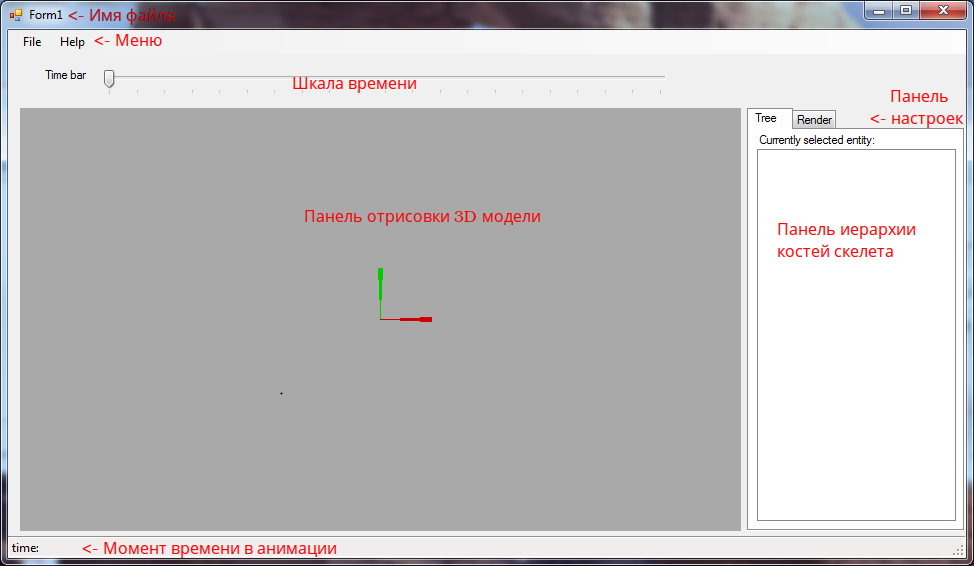
\includegraphics[width=0.8\textwidth]{../screenshots/main_empty.png}
    \caption{Схема интерфейса}
\end{figure}


\newpage
\section{Приложение 3. Список используемой литературы}
\subsection{Список используемой литературы}
\begin{my_enumerate}
\item
ГОСТ 19.101-77 Виды программ и программных документов
//Единая система программной документации. -М.: ИПК Издательство стандартов, 2.: 001.

\item
ГОСТ 19.103-77 Обозначения программ и программных документов. //Единая система программной документации. -М.: ИПК Издательство стандартов, 2001.

\item
ГОСТ 19.104-78 Основные надписи //Единая система программной документации. -М.: ИПК Издательство стандартов, 2001.

\item 
ГОСТ 19.105-78 Общие требования к программным документам. //Единая система
программной документации. – М.: ИПК Издательство стандартов, 2001.

\end{my_enumerate}



% Index
\newpage
\eskdListOfChanges

% \phantomsection
% \addcontentsline{toc}{section}{Алфавитный указатель}
% \printindex

\end{document}
